\documentclass[lecture.tex]{subfiles}

\begin{document}

\exercice{}
%\video{https://youtu.be/blablabla}
\enonce{rdm-0005}{Treillis 3 barres}


\begin{center}
  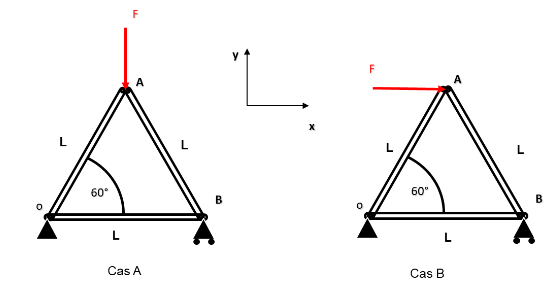
\includegraphics[scale=0.5]{exo-treillis-3-barres.png}
\end{center}

Pour les deux cas ci-dessus :

\begin{enumerate}
  \item Faire le bilan des actions mécaniques extérieures à la poutre.
  \item Déterminer le degré d’hyperstatisme de la poutre.
  \item Trouver les inconnus de liaison de la structure (les efforts et les moments résultants de l’encastrement).
\end{enumerate}

\finenonce{rdm-0005}
\finexercice

\end{document}
